% Illustrative schematic only. Positions and ratings are not taken from any reviewed source.
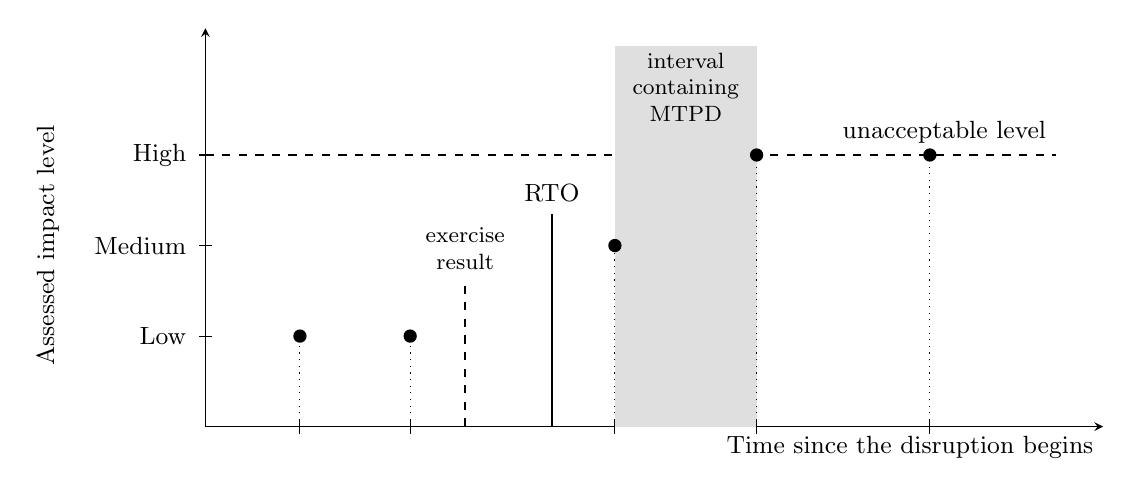
\begin{tikzpicture}[x=1cm,y=1.15cm,>=stealth,font=\small]
  % Axes
  \draw[->] (0,0) -- (11.4,0) node[below left] {Time since the disruption begins};
  \draw[->] (0,0) -- (0,4.4);
  \foreach \y/\l in {1/Low,2/Medium,3/High}{
    \draw (-0.08,\y) -- (0.08,\y);
    \node[left] at (-0.12,\y) {\l};
  }
  \node[rotate=90] at (-2.0,2) {Assessed impact level};
  % Unacceptable level
  \draw[dashed] (0,3) -- (10.8,3);
  \node[above left] at (10.8,3.02) {unacceptable level};
  % Interval that contains the MTPD
  \fill[gray!25] (5.2,0) rectangle (7.0,4.2);
  \node[align=center,font=\footnotesize] at (6.1,3.75) {interval\\containing\\MTPD};
  % Assessed points
  \foreach \x/\y in {1.2/1,2.6/1,5.2/2,7.0/3,9.2/3}{
    \fill (\x,\y) circle (2.4pt);
    \draw[dotted] (\x,0) -- (\x,\y);
    \draw (\x,-0.08) -- (\x,0.08);
  }
  % Recovery time objective and demonstrated recovery time
  \draw[thick] (4.4,0) -- (4.4,2.35);
  \node[above] at (4.4,2.38) {RTO};
  \draw[thick,dashed] (3.3,0) -- (3.3,1.6);
  \node[above,align=center,font=\footnotesize] at (3.3,1.63) {exercise\\result};
\end{tikzpicture}